
\documentclass[12pt]{exam}
\usepackage{amsthm}
\usepackage{libertine}
%\usepackage[utf8]{inputenc}
\usepackage[margin=1in]{geometry}
\usepackage{amsmath,amssymb}
\usepackage{multicol}
\usepackage[shortlabels]{enumitem}
\usepackage{siunitx}
\usepackage{cancel}
\usepackage{graphicx}
\graphicspath{{./}}
\usepackage{pgfplots}
\usepackage{hyperref}
\usepackage{listings}
\usepackage{tikz}
\usepackage{minted}
\def\code#1{\texttt{#1}}
\usepackage{amssymb}
\usepackage{xcolor}
% for plotting
\usepackage{pgfplots}
\pgfplotsset{compat=1.16}
\usepackage{tikz}
\usetikzlibrary{arrows.meta}

\newcommand{\quotebox}[1]
{
  \begin{center}
    \fcolorbox{white}{blue!15!gray!15}{
      \begin{minipage}{0.7\linewidth}\vspace{10pt}
        \center
        \begin{minipage}{0.8\linewidth}{\space\Huge``}{\setlength{\parindent}{1.5em}#1}{\hspace{1.5em}\break\null\Huge\hfill''}
        \end{minipage}
        \smallbreak
      \end{minipage}
    }
\end{center}
}

%\DeclareUnicodeCharacter{2212}{-}


\let\oldemptyset\emptyset
\let\emptyset\varnothing

\hypersetup{
    colorlinks=true,
    linkcolor=blue,
    filecolor=magenta,      
    urlcolor=cyan,
    pdftitle={Overleaf Example},
    pdfpagemode=FullScreen,
    }
    
\urlstyle{same}

\pgfplotsset{width=10cm,compat=1.9}
\usepgfplotslibrary{external}
\tikzexternalize

\newcommand{\class}{Math 415} % This is the name of the course 
\newcommand{\examnum}{Homework-8} % This is the name of the assignment
\newcommand{\examdate}{Nov 16} % This is the due date
\newcommand{\timelimit}{}

\newcommand{\BO}{\mathcal{O}}




\begin{document}
\pagestyle{plain}
\thispagestyle{empty}

\noindent
\begin{tabular*}{\textwidth}{l @{\extracolsep{\fill}} r @{\extracolsep{6pt}} l}
\textbf{\class} & \textbf{Name:} & \textit{Zhenzhao Tu}\\ %Your name here instead, obviously 
\textbf{\examnum} &&\\
\textbf{\examdate} &&\\
\end{tabular*}\\
\rule[2ex]{\textwidth}{2pt}
% --



\section*{Problem 1}
Consider the nonlinear oscillator
\[ \ddot{x} + a\dot{x}(x^2+ \dot{x}^2-1) + x = 0 \]
where $a$ is in $(0,2)$. 

\begin{enumerate}[(a)]
    \item Let $y = \dot{x}$. Show that the system can be written as a first order system
	    \[ \begin{cases}
		    \dot{x} = y \\
		    \dot{y} = -ay(x^2+y^2-1) - x
		    \end{cases}. \]
	To find the fixed points, we need to solve the system when $\dot{x} = \dot{y} = 0$. So we have
	\[ \begin{cases}
		y = 0 \\
		-ay(x^2+y^2-1) - x = 0
		\end{cases} \]
	which implies $x = 0$ and $y=0$ thus the fixed point is $(0,0)$.

    \item Let $(x,y) = (r\cos\theta, r\sin\theta)$. Show that the system can be written as
	    \[ \begin{cases}
		    \dot{r} = -ar(\sin\theta)^2(r^2-1) \\
		    \dot{\theta} = -1 - a \sin \theta \cos \theta (r^2-1)
		    \end{cases} \]
	    thus this is a polar system.\\
	    When $\dot{r} = 0$, we have $r = 0$ or $r = \pm 1$. Since the radius cannot be negative and zero, so when $r=1$ we have a circular limit cycle. The amplitude of the limit cycle is $1$ and period is $2\pi$.

    \item By linearizing the radius about $1$, we have $r(t) = A+ \delta(t) = 1 + \delta(t)$. Then we have
	    \[ \dot{\delta} = -a(1+\delta)(\sin\theta)^2((\delta +1)^2 - 1) \]
	    Since $\delta \ll 1$, we can ignore the higher order terms in Taylor expansion. Thus we can approximate the $(\delta + 1)^2 \approx 1 + 2\delta$. Then we have
	    \[ \dot{\delta} \approx -a(1+\delta)(\sin\theta)^2(2\delta) = -2ar \sin^2\theta \delta \]
	   Now we can see that $\dot{\delta}$ is linear and less than zero, so the limit cycle is stable.
	      

\end{enumerate}


\section*{Problem 2}
Show the following system are gradient systems

\begin{enumerate}[(a)]
	\item For the first system
	\[ \dot{x} = y^2 + y \cos x, \quad \dot{y} = 2xy + \sin y. \]
	Now we test $\partial V/ \partial x = - f(x, y )$ we have
	\begin{align*}
		\frac{\partial V}{\partial x} &= -y^2 - y \cos x \\
		\int \frac{\partial V}{\partial x}  &= -y^2 x - y \sin x + C 
	\end{align*}
	Then we test $\partial V/ \partial y = - g(x, y )$ we have
	\begin{align*}
		\frac{\partial V}{\partial y} &= -2xy - \sin y \\
		\int \frac{\partial V}{\partial y}  &= -y^2 x - y\sin x + C
	\end{align*}
	Thus we can find a potential function $V(x,y) = -y^2 x - y \sin x$ such the conditions. So the system is a gradient system.

	\item For the second system
		\[ \dot{x} = 3x^2 -1-e^{2y}, \quad \dot{y} = -2 x e^{2y} \]
		Now we test $\partial V/ \partial x = - f(x, y )$ we have
		\begin{align*}
			\frac{\partial V}{\partial x} &= -3x^2 + 1 + e^{2y} \\
			\int \frac{\partial V}{\partial x}  &= -x^3 + x + e^{2y}x + C
		\end{align*}
		Then we test $\partial V/ \partial y = - g(x, y )$ we have
		\begin{align*}
			\frac{\partial V}{\partial y} &= 2xe^{2y} \\
			\int \frac{\partial V}{\partial y}  &= xe^{2y} + C_y
		\end{align*}
		Where the $C_y = -x^3+x$. Thus we can find a potential function $V(x,y) = -x^3 + x + e^{2y}x$ such the conditions. So the system is a gradient system.
\end{enumerate}

\section*{Problem 3}
Show that the system $\dot{x} = y -x^3$, $\dot{y} = -x -y^3$ has no closed orbits.

\begin{proof}
	By constructing a Lyapunov function $V(x,y) = ax^2 + by^2$, we can form a suitable $a,b$ for the system. Then we have $\dot{V}(x,y) = 2ax\dot{x} + 2by\dot{y}$, by substituting the system we have
	\begin{align*}
		\dot{V}(x,y) &= 2ax(y-x^3) + 2by(-x-y^3) \\
		&= 2axy - 2ax^4 - 2bxy - 2by^4 \\
		&= 2xy(a-b) - 2x^4a - 2y^4b
	\end{align*}
	When $a=b > 0$, we have $\dot{V}(x,y) = -2x^4a - 2y^4b < 0$. Thus the system is stable. Since the system is stable, so there is no closed orbits.
\end{proof}



\section*{Problem 4}
Consider the system $\dot{x} = x^2 -y-1$, $\dot{y} = y(x-2)$.
\begin{enumerate}[(a)]
	\item Let $\dot{x} = 0$, $\dot{y} = 0$, we have $x^2 - y - 1 = 0$ and $y(x-2) = 0$. Thus we have $y = 0$ or $x = 2$. When $y = 0$, we have $x = \pm 1$. When $x = 2$, we have $y = 3$. Thus the fixed points are $(-1,0)$, $(1,0)$ and $(2,3)$. Then let's find the jacobian matrix of the system
	\[ J = \begin{bmatrix}
		2x & -1 \\
		y & x-2
	\end{bmatrix} \]
	Then we can evaluate the jacobian matrix at the fixed points. For three fixed points $(-1,0)$, $(1,0)$ and $(2,3)$, we have the jacobian matrix respectively
	\[ J_{(-1,0)} = \begin{bmatrix}
		-2 & -1 \\
		0 & -3
	\end{bmatrix}, \quad J_{(1,0)} = \begin{bmatrix}
		2 & -1 \\
		0 & -1
	\end{bmatrix}, \quad J_{(2,3)} = \begin{bmatrix}
		4 & -1 \\
		3 & 0
	\end{bmatrix} \]
	Based on the jacobian matrix, we can find the eigenvalues of the fixed points. For $(-1,0)$, we have $\lambda_1 = -2$ and $\lambda_2 = -3$. For $(1,0)$, we have $\lambda_1 = 2$ and $\lambda_2 = -1$. For $(2,3)$, we have $\lambda_1 = 3$ and $\lambda_2 = 1$. Thus we can see that $(1,0)$ is a saddle point, $(-1,0)$ is a stable node and $(2,3)$ is a unstable node.

\item Let's call $A= (-1,0)$, $B = (1,0)$ and $C = (2,3)$. Then let's find lines $AB$, $BC$ and $AC$. By simple calculation, we have $l_{AB}: y = 0$, $l_{BC}: y = 3x-3$ and $l_{AC}: y = x+1$. Then we can examine these lines see if they are invariant. 
	\begin{enumerate}[(i)]
		\item For $l_{AB}$, we can substitute $y=0$ into the system and we have $\dot{x} = x^2 - 1$ and $\dot{y} = 0$. Then we can see that $\dot{x} < 0$ when $x \in [-1,1]$. Thus the line $l_{AB}$ is invariant.
		\item For $l_{BC}$, we can substitute $y=3x-3$ into the system and we have $\dot{x} = x^2 - 3x + 2 = (x-2)(x-1)$ and $\dot{y} = 3(x-1)(x-2)$. Thus $\dot{y} = 3\dot{x}$. Since the slope of $\dot{y}$ is same as $y$, we know that every point on the line $l_{BC}$ will move along the line $l_{BC}$. Thus the line $l_{BC}$ is invariant. 
		\item For $l_{AC}$, we can substitute $y=x+1$ into the system and we have $\dot{x} = x^2 - x - 2 = (x-2)(x+1)$ and $\dot{y} = (x-2)(x+1)$. Thus $\dot{y} = \dot{x}$. Since the slope of $\dot{y}$ is same as $y$, we know that every point on the line $l_{AC}$ will move along the line $l_{AC}$. Thus the line $l_{AC}$ is invariant.
	\end{enumerate}

	\item Here is the phase portrait of the system. The red circle is the closed curve at $(-1, 0)$, the blue circle is the closed curve at $(1,0)$ and the green circle is the closed curve at $(2,3)$.
	\begin{figure}[H]
		\centering
		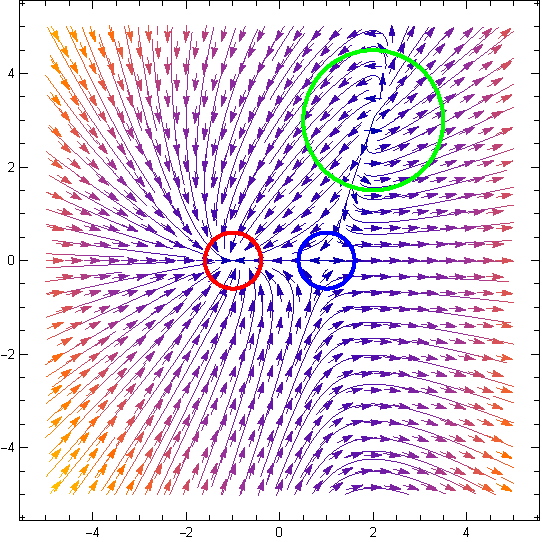
\includegraphics[width=0.6\linewidth]{4c.pdf}
		\caption{Phase portrait of the system}
		\label{fig:phase}
	\end{figure}
	For those three closed curves are all violates the rule that trajectories cannot cross becasue there is always straight line between two fixed points. Thus the system cannot had a closed orbit.
\end{enumerate}

\section*{Problem 5}
Consider the system 
\[ \begin{cases}
	\dot{x} = x - y -x(x^2+5y^2) \\
	\dot{y} = x +y - y(x^2+y^2)
\end{cases} \]

\begin{enumerate}[(a)]
	\item Let $\dot{x} = 0$, $\dot{y} = 0$, we have $x - y -x(x^2+5y^2) = 0$ and $x +y - y(x^2+y^2) = 0$. Thus we have $(x^*, y^*) = (0, 0)$. Then let's find the jacobian matrix of the system at $(0,0)$
	\[ J = \begin{bmatrix}
		1-3x^2-5y^2 & -1-10xy \\
		1-2xy & 1-x^2-3y^2
	\end{bmatrix}_{(0,0)} = \begin{bmatrix}
		1 & -1 \\
		1 & 1
	\end{bmatrix} \]
	Then we can find the eigenvalues of the fixed point $(0,0)$, we have $\lambda_1 = 1 + i$ and $\lambda_2 = 1 - i$. Thus we can see that $(0,0)$ is a unstable spiral node. 

	\item Let $(x,y) = (r\cos\theta, r\sin\theta)$. Show that the system can be written as
		\[ \begin{cases}
			\dot{r} = r-r^3 -2r^3 \sin^2\theta \cos^2\theta \\
			\dot{\theta} = 1 + 4r^2 \sin^3\theta \cos\theta
		\end{cases} \]
		thus this is a polar system.
		
	\item Consider $r_1$ as the radius for inner circle, $r_2$ as the radius for outer circle. Then for $r_1$ must such that $\dot{r} >0$ and for $r_2$ must such that $\dot{r} < 0$. Thus we have
		\[ \begin{cases}
			r_1 - r_1^3 - 2r_1^4 \sin^2\theta \cos^2\theta > 0 \\
			r_2 - r_2^3 - 2r_2^4 \sin^2\theta \cos^2\theta < 0
		\end{cases} \]
		Then we can solve the inequality and we have $r_1 \in (1/\sqrt{3}, 1)$ and $r_2 \in (1/\sqrt{3}, \infty)$. Thus the largest $r_1$ is $1$ and the smallest $r_2$ is $1/\sqrt{3}$.
\end{enumerate}











\end{document}

